\textbf{Supplementary}

\section{Extended Machine Learning Discussion}

\subsection{Reproducible Plots}
In this section, we put reproducible plots and will update the plots when we get full results. 

\begin{figure}[h]
    \centering
    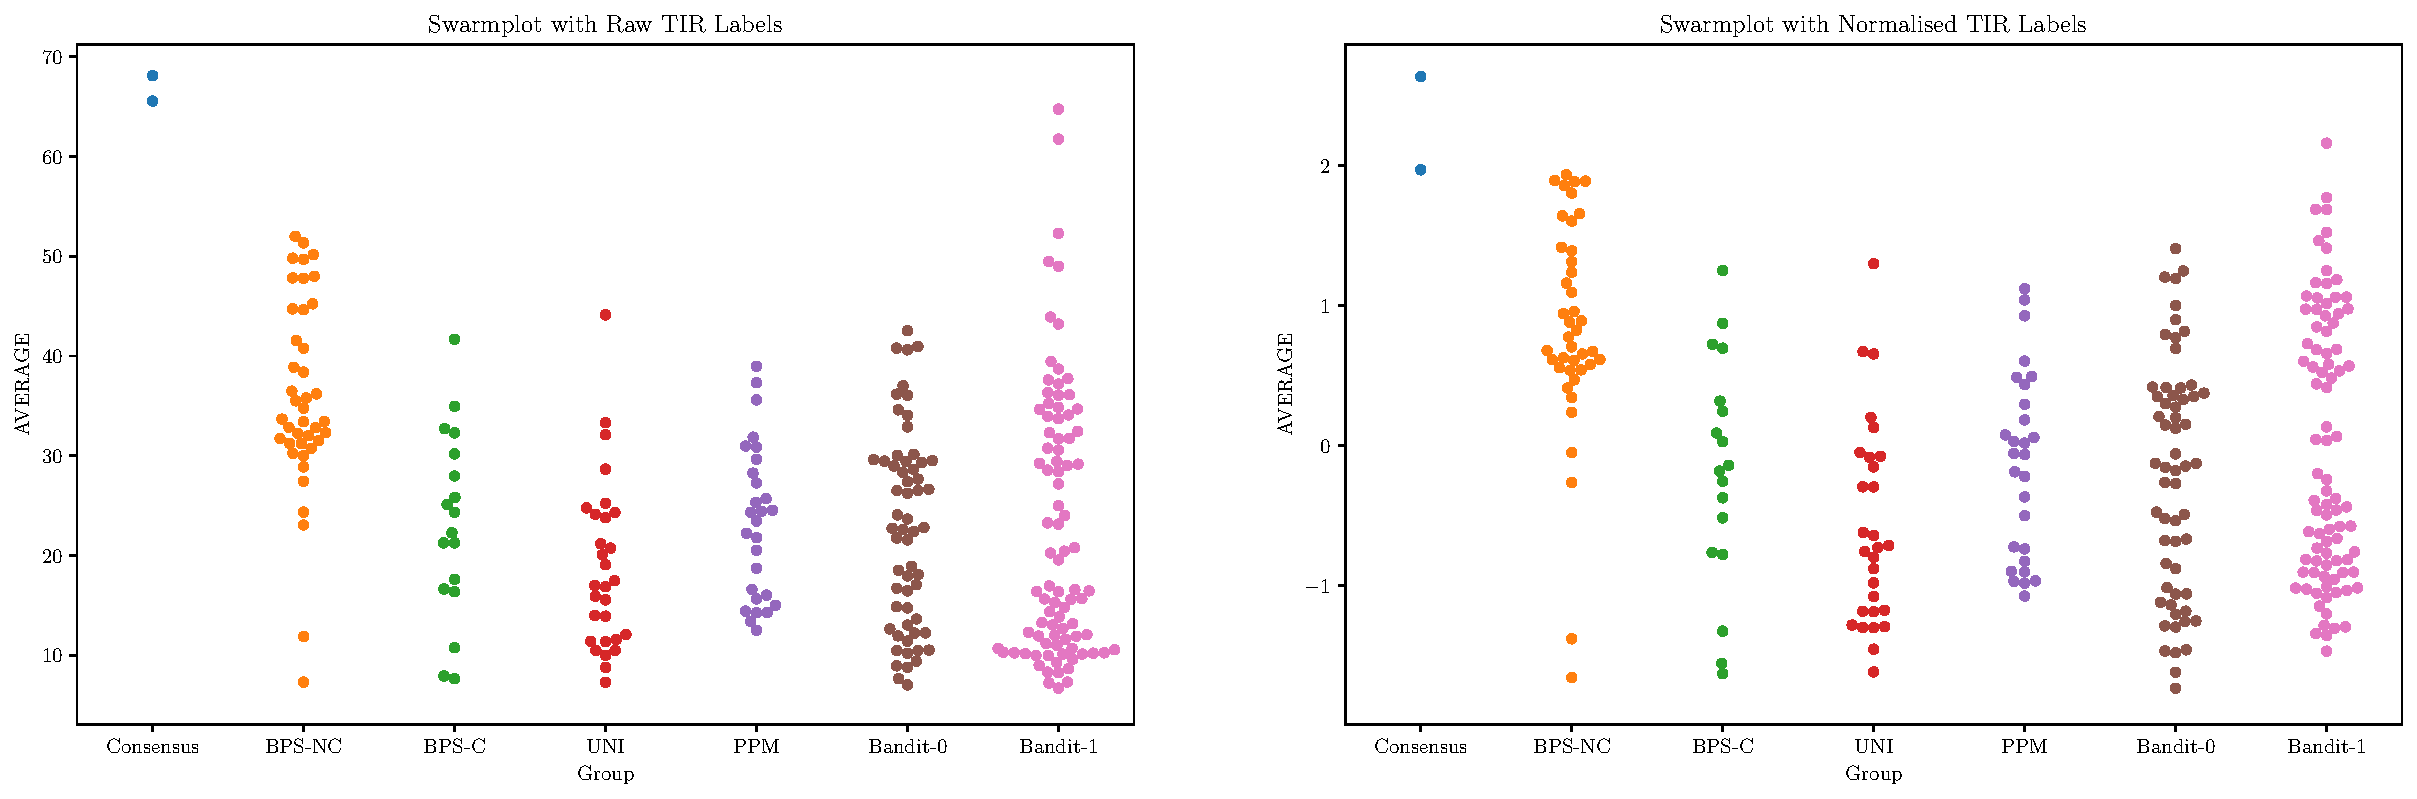
\includegraphics[scale = 0.4]{plots/Supplementary/swarmplots.pdf}
    \caption{Swarmplots for different groups, with raw (left) and normalised (right) TIR labels (averaged over 6 replicates). 
    Group names represent: Consensus (consensus sequence tested in different round); BPS-NC (bps noncore); BPS-C (bps core); UNI (uniformly random); PPM (position-based probability matrix); Bandit-0 (bandit design for round 0); Bandit-1 (bandit design for round 1).}
    \label{fig:swarmplots.}
\end{figure}

\begin{figure}
    \centering
    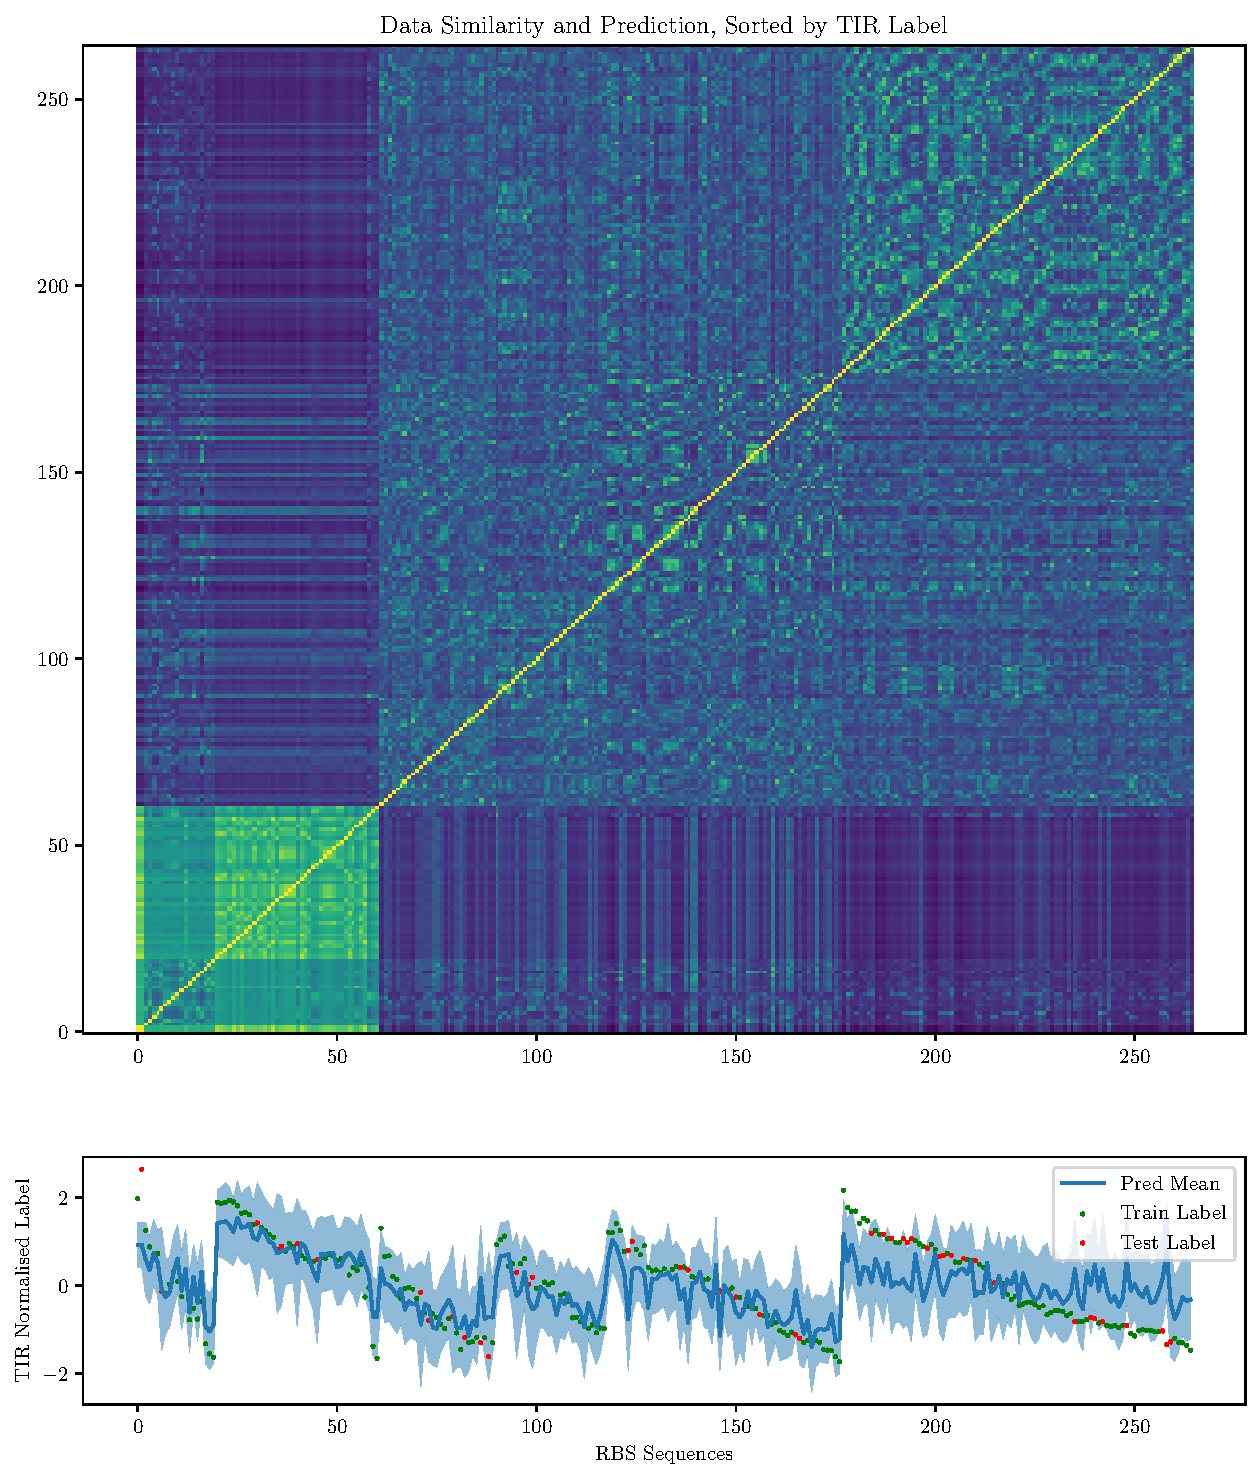
\includegraphics[scale = 0.3]{plots/Supplementary/Data_Similarity_and_Prediction_Sorted_by_TIR_Label.pdf}
    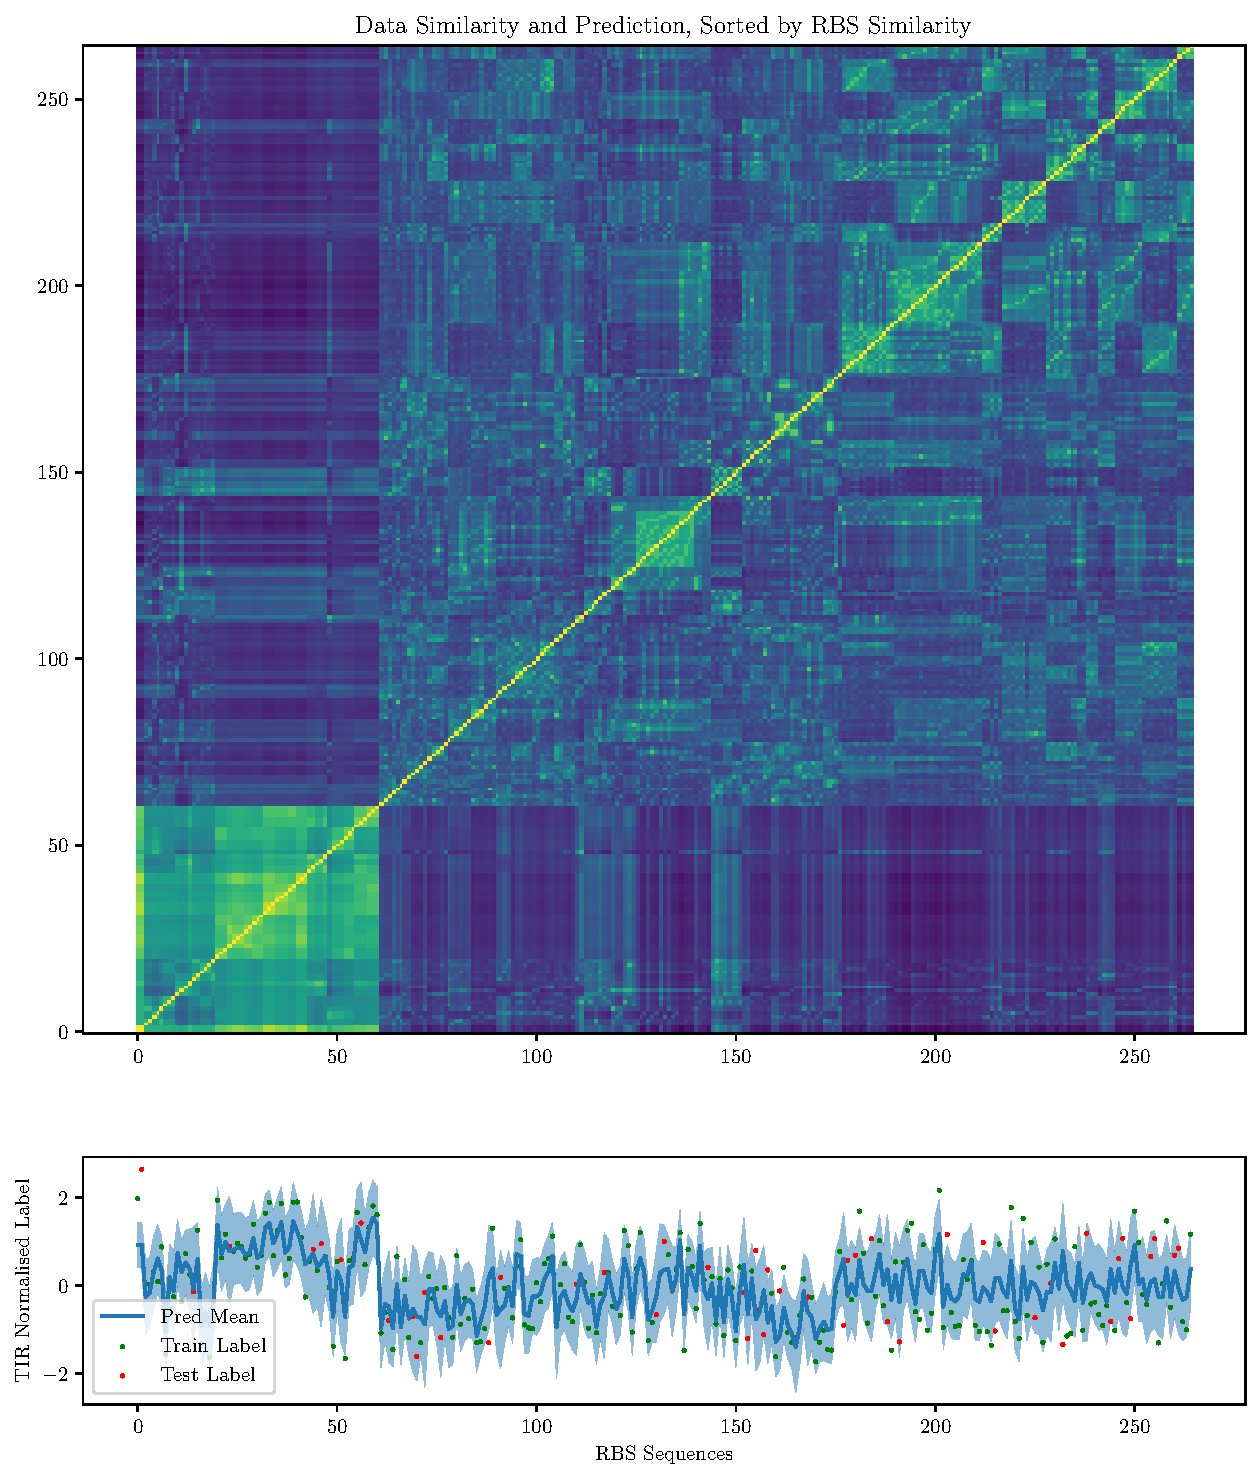
\includegraphics[scale = 0.3]{plots/Supplementary/Data_Similarity_and_Prediction_Sorted_by_RBS_Similarity.pdf}
    \caption{Kernel Heatmap and Predictions. Sequences are grouped as Consensus (1-2), BPS-C (3-20), BPS-NC (21-61), UNI (62-90), PPM (91-118), Bandit-0 (119-177), Bandit-1 (178-265). Inside of each group, sequences are clustered and sorted in terms of TIR labels (left) or RBS similarity (right). The first row shows the similarity measured by weighted degree kernel with shift, the second shows the predicted mean and uncertainty (1.95 standard deviation).}
    \label{fig:my_label}
\end{figure}

\begin{figure}
    \centering
    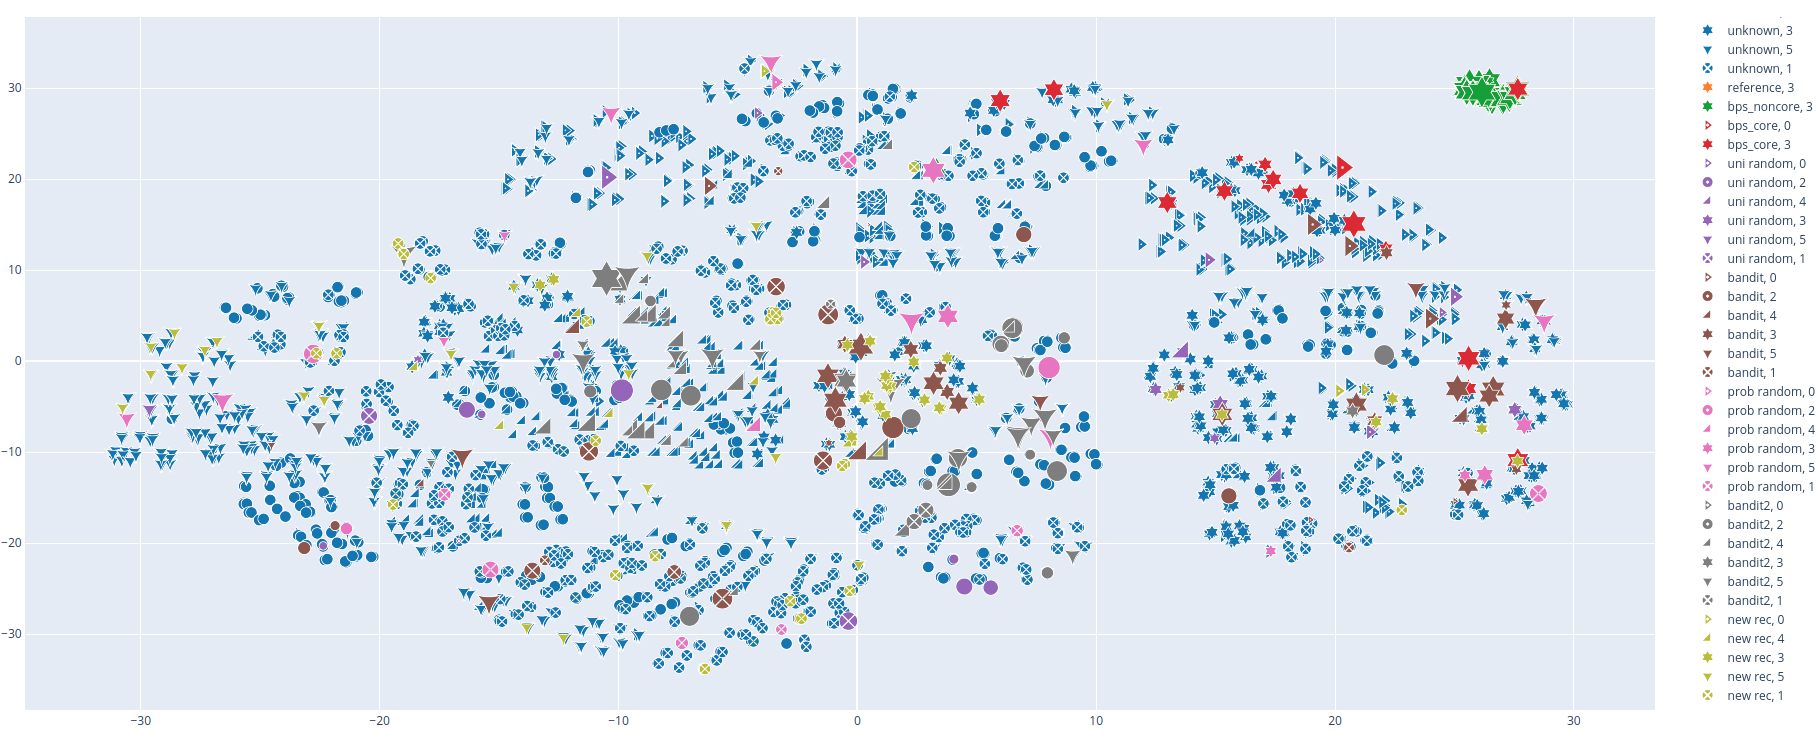
\includegraphics[scale = 0.25]{plots/Supplementary/clustering.png}
    \caption{TSNE of RBS sequences in design space with clustering. The distance is calculated based on the weighted degree kernel on RBS sequences. Colours indicate different groups, shapes indicate different clusters.}
    \label{fig:my_label}
\end{figure}

\subsection{Gaussian Process Regression}

A \textit{Gaussian process} is a collection of random variables, any finite number of which have a joint Gaussian distribution. 
We define mean function $\mu(\mathbf{x})$  and covariance function $k(\mathbf{x}, \mathbf{x}^\prime)$ of a real process $f(\mathbf{x})$ as
\begin{align}
    \mu(\mathbf{x}) &= \mathbb{E}[f(\mathbf{x})]\\
    k(\mathbf{x}, \mathbf{x}^\prime) &= \mathbb{E}[(f(\mathbf{x}) - \mu(\mathbf{x}))(f(\mathbf{x}^\prime) - \mu(\mathbf{x}^\prime))].
\end{align}

A Gaussian process is specified by its mean function and convariance function as $f(\mathbf{x}) \sim \mathcal{G} \mathcal{P}\left(\mu(\mathbf{x}), k\left(\mathbf{x}, \mathbf{x}^{\prime}\right)\right)$.
We consider the case where the observations are noisy, i.e. $\{(\mathbf{x}_i, y_i)| i = 1, \dots, n\}$, where $y_i = f(\mathbf{x}_i) + \epsilon$ with $\epsilon \sim \mathcal{N}(0, \alpha^2)$. 
The Gaussian noise is independent identically distributed, and the prior on the noisy observations is then $\operatorname{cov}\left(y_{p}, y_{q}\right)=k\left(\mathbf{x}_{p}, \mathbf{x}_{q}\right)+\alpha^{2} \delta_{p q}$,
where $\delta_{pq}$ is a Kronecker delta which is one if $p = q$ and zero otherwise.
It is equivalent to a diagonal matrix $\alpha^2 I$ on the kernel matrix evaluated on the training points.

For $n_\ast$ test points $X_\ast$, we assume the prior over the functions values as a random Gaussian vector $\mathbf{f}_\ast \sim \mathcal{N}(\mathbf{0}, K(X_\ast, X_\ast))$.
Then the joint distribution of the observed target values and the function values at the test points under the prior as 
\begin{align}
    \left[\begin{array}{l}\mathbf{y} \\ \mathbf{f}_{*}\end{array}\right] \sim \mathcal{N}\left(\mathbf{0},\left[\begin{array}{cc}K(X, X)+\alpha^{2} I & K\left(X, X_{*}\right) \\ K\left(X_{*}, X\right) & K\left(X_{*}, X_{*}\right)\end{array}\right]\right)
\end{align}
where $K(X, X_\ast)$ denotes the $n \times n_\ast$ covariance/Kernel matrix evaluated at all pairs of training and testing points, similarly for other kernel matrices.
Then the posterior of the test points (i.e. predictive distributions) is given by the conditional distribution $\mathbf{f}_\ast | X, \mathbf{y}, X_\ast \sim \mathcal{N}(\bar{\mathbf{f}}_\ast, cov(\mathbf{f}_\ast))$, where
\begin{align}
   \overline{\mathbf{f}}_{*} & \triangleq \mathbb{E}\left[\mathbf{f}_{*} \mid X, \mathbf{y}, X_{*}\right]=K\left(X_{*}, X\right)\left[K(X, X)+\alpha^{2} I\right]^{-1} \mathbf{y} \\
   \label{Eq: predicted variance}
   \operatorname{cov}\left(\mathbf{f}_{*}\right) &=K\left(X_{*}, X_{*}\right)-K\left(X_{*}, X\right)\left[K(X, X)+\alpha^{2} I\right]^{-1} K\left(X, X_{*}\right) 
\end{align}
For noisy test targets $\mathbf{y}_\ast$, we can compute the predictive distribution by adding $\alpha^2 I$ to the variance term $cov(\mathbf{f}_\ast)$ in Eq. (\ref{Eq: predicted variance}).
% We now introduce the marginal likelihood (or evidence) $p(\mathbf{y}|X)$, is which the integral of the likelihood times the prior 
% \begin{align}
%     p(\mathbf{y} \mid X)=\int p(\mathbf{y} \mid \mathbf{f}, X) p(\mathbf{f} \mid X) d \mathbf{f}
% \end{align}



\subsection{Choices of Kernels}

The choice of covariance function is critical for the performance of Gaussian process regression, we show a number of different string kernels tested in this study below:

\begin{itemize}
    \item \textit{Spectrum Kernel.}
    \begin{align}
        k_\ell^{\text{Spec}}(X, X^\prime) =\left\langle\phi_{\ell}^{\mathrm{Spec}}(\mathbf{x}), \phi_{\ell}^{\mathrm{Spec}}\left(\mathbf{x}^{\prime}\right)\right\rangle = \phi_{\ell}^{\mathrm{Spec}}(\mathbf{x})^T \phi_{\ell}^{\mathrm{Spec}}\left(\mathbf{x}^{\prime}\right).
    \end{align}
     where $\mathbf{x}, \mathbf{x}^\prime$ are two RBS sequences in $\mathcal{D}$ over an alphabet $\Sigma$. We denote the number of letters in the alphabet as $|\Sigma|$. 
    $\phi_{\ell}^{\mathrm{spec}}(\mathbf{x})$ maps the sequence $X$ into a $|\Sigma|^\ell$ dimensional feature space, where each dimension is the count of the number of one of the $|\Sigma|^\ell$ possible strings $s$ of length $\ell$. 
    Let $X, X^\prime$ be two metrics which include $n$ sequences, and $\Phi_d^{Spec}(X) \in \mathbb{R}^{n \times |\Sigma|^{\ell}}$, then the spectrum kernel over metrics is 
    \begin{align}
         K_\ell^{\text{Spec}}(X, X^\prime) = \Phi_{\ell}^{\mathrm{Spec}}(X) \Phi_{\ell}^{\mathrm{Spec}}\left(X^{\prime}\right)^T.
    \end{align}
    
    \item \textit{Sum of Spectrum Kernel,} considers weighted sum over different parts of the string. 
    
    \item \textit{Mixed Spectrum Kernel,} considers weighted sum over different substring length, with $\beta_d = \frac{2(\ell - d + 1)}{\ell(\ell+1)}$,
        \begin{align}
            k_\ell^{MixedSpec}(\mathbf{x}, \mathbf{x}^\prime) 
            = \sum_{d=1}^{\ell} \beta_d k_d^{Spec}(\mathbf{x}, \mathbf{x}^\prime)
        \end{align}
    \item \textit{Weighted Degree Kernel,} considers positional information. WD kernel counts the match of kmers at corresponding positions in two sequences.
    For sequences with fixed length $L$ and weighted degree kernel considers substrings starting at each position $l = 1, ..., L$, with $\beta_d = \frac{2(\ell - d + 1)}{\ell(\ell+1)}$, \\
    \begin{align}
        k_\ell^{WD}(\mathbf{x}, \mathbf{x}^\prime) 
        &= \sum_{d=1}^{\ell} \beta_d \sum_{l=1}^{L-d+1} \gamma_l k_d^{Spec}(\mathbf{x}_{[l:l+d]}, \mathbf{x}_{[l:l+d]}^\prime)\\
        &= \sum_{d=1}^{\ell} \beta_d \sum_{l=1}^{L-d+1} \gamma_l \phi_d^{Spec}(\mathbf{x}_{[l:l+d]})^T \phi_d^{Spec}(\mathbf{x}_{[l:l+d]}^\prime)\\
        &= \sum_{d=1}^{\ell} \beta_d \sum_{l=1}^{L-d+1} \gamma_l \mathbb{I}(\mathbf{x}_{[l:l+d]} = \mathbf{x}_{[l:l+d]}^\prime),
    \end{align}
    where $\mathbb{I}(\text{true}) = 1$ and 0 otherwise. 
    
    \item \textit{Weighted Degree Kernel With Shift.}
    \begin{align}
        k_\ell^{WDS}(\mathbf{x}, \mathbf{x}^\prime) 
        &= \sum_{d=1}^{\ell} \beta_d \sum_{l=1}^{L-d+1} \gamma_l \sum_{s = 0, s + l \leq L}^{S(l)} \delta_s
        \left(k_d^{Spec}(\mathbf{x}_{[l+s:l+s+d]}, \mathbf{x}_{[l:l+d]}^\prime) + (k_d^{Spec}(\mathbf{x}_{[l:l+d]}, \mathbf{x}_{[l+s:l+s+d]}^\prime)\right)\\
        &= \sum_{d=1}^{\ell} \beta_d \sum_{l=1}^{L-d+1} \gamma_l \sum_{s = 0, s + l \leq L}^{S(l)} \delta_s
        \left(\mathbb{I}(\mathbf{x}_{[l+s:l+s+d]} = \mathbf{x}_{[l:l+d]}^\prime) + (\mathbb{I}(\mathbf{x}_{[l:l+d]}= \mathbf{x}_{[l+s:l+s+d]}^\prime)\right),
    \end{align}
    where $\beta_d = \frac{2(\ell - d + 1)}{\ell(\ell+1)}, \delta_s = \frac{1}{2(s+1)}$, $\gamma_l$ is a weighting over the position in the
    sequence, where we choose to use a uniform weighting over the sequences, i.e. $\gamma_l = 1/L$. $S(l)$ determines the shift
    range at position $l$.
\end{itemize}

\textbf{From kernel to distance}:
$$d(\mathbf{x}, \mathbf{x}^\prime) = \sqrt{k(\mathbf{x}, \mathbf{x}) + k(\mathbf{x}^\prime, \mathbf{x}^\prime) - 2 k(\mathbf{x}, \mathbf{x}^\prime)} $$

\subsubsection{Normalisation of Kernel}

As part of data pre-processing,
the range of all features should be normalised so that each feature contributes approximately proportionately to the predictive model. 
The kernel matrix is represented by the inner product of the underlying feature vectors, it needs to be normalised before being used in the downstream regression models. 
Up-scaling (down-scaling) features can be understood as down-scaling (up-scaling) regularizers such that they penalise the features less (more). 

Here we consider two approaches for kernel normalisation: centering and unit norm. 
We will show how to convert the normalisation in terms of feature vectors to normalisation in terms of kernel matrices. 
As defined before, consider $\mathbf{x}, \mathbf{x}^\prime$ are two RBS sequences in $\mathcal{D}$ over an alphabet $\Sigma$.
We denote $\phi(\mathbf{x}_i)$ as a column feature vector of sequence $\mathbf{x}_i$, 
where a feature function $\phi: \mathbf{x} \rightarrow \mathbb{R}^d$. Assume there is total of $n$ sequences in the data $X$ ($n'$ sequences in the data $X'$). 
We illustrate centering and unit norm normalisation below. 

\begin{itemize}
    \item Centering. 
    Defining the mean vector as $\bar{\Phi}(X) = \frac{1}{n} \sum_{s = 1}^n \phi(\mathbf{x}_s) \in \mathbb{R}^d$, the centered feature vector $\phi^C(\mathbf{x}_i) \in \mathbb{R}^d$ of $\mathbf{x}_i$ is
    \begin{align}
        \phi^{C}(\mathbf{x}_i) = \phi(\mathbf{x}_i) - \bar{\Phi}(X) = \phi(\mathbf{x}_i) - \frac{1}{n'} \sum_{s = 1}^{n'} \phi(\mathbf{x}_s).
    \end{align}
    The corresponding centering kernel value between $\mathbf{x}_i$ and $\mathbf{x}_j$ is then 
    \begin{align}
        k^C(\mathbf{x}_i, \mathbf{x}_j) &= <\phi^C(\mathbf{x}_i), \phi^C(\mathbf{x}_j)>\\
        &= \left( \phi(\mathbf{x}_i) - \frac{1}{n} \sum_{s = 1}^n \phi(\mathbf{x}_s)\right)^T \left( \phi(\mathbf{x}_j) - \frac{1}{n'} \sum_{s' = 1}^{n'} \phi(\mathbf{x}_{s'})\right)\\
        &= \phi(\mathbf{x}_i)^T \phi(\mathbf{x}_j) - \left( \frac{1}{n} \sum_{s = 1}^n \phi(\mathbf{x}_s)\right)^T \phi(\mathbf{x}_j) - \phi(\mathbf{x}_i)^T \left(\frac{1}{n} \sum_{s' = 1}^{n'} \phi(\mathbf{x}_{s'})\right) + \left( \frac{1}{n} \sum_{s = 1}^n \phi(\mathbf{x}_s)\right)^T \left(\frac{1}{n'} \sum_{s' = 1}^{n'} \phi(\mathbf{x}_{s'})\right)\\
        &= k(\mathbf{x}_i, \mathbf{x}_j) - \frac{1}{n} \sum_{s=1}^n k(\mathbf{x}_s, \mathbf{x}_j) - \frac{1}{n'} \sum_{s'=1}^{n'} k(\mathbf{x}_i, \mathbf{x}_{s'}) + \frac{1}{n^2} \sum_{s = 1}^n \sum_{s'=1}^{n'} k(\mathbf{x}_s, \mathbf{x}_{s'})
    \end{align}
    
    \item Unit Norm. Define the ($l_2$) norm of a feature vector as $||\phi(\mathbf{x})|| = \sqrt{\sum_{m = 1}^d \phi_d(\mathbf{x})^2} = \sqrt{k(\mathbf{x}, \mathbf{x})} \in \mathbb{R}^+$, then the unit norm feature vector $\phi^{UN}(\mathbf{x}_i) \in \mathbb{R}^d$ of $\mathbf{x}_i$ is 
    \begin{align}
        \phi^{UN}(\mathbf{x}_i) = \frac{\phi(\mathbf{x}_i)}{||\phi(\mathbf{x}_i)||}.
    \end{align}
    The corresponding unit norm kernel value between $\mathbf{x}_i$ and $\mathbf{x}_j$ is then 
    \begin{align}
        k^{UN}(\mathbf{x}_i, \mathbf{x}_j) &= <\frac{\phi(\mathbf{x}_i)}{||\phi(\mathbf{x}_i)||}, \frac{\phi(\mathbf{x}_j)}{||\phi(\mathbf{x}_j)||}>\\
        &= \frac{\phi(\mathbf{x}_i)^T \phi(\mathbf{x}_j)}{||\phi(\mathbf{x}_i)|| \times ||\phi(\mathbf{x}_j)||}\\
        &= \frac{k(\mathbf{x}_i, \mathbf{x}_j)}{\sqrt{k(\mathbf{x}_i, \mathbf{x}_i)  k(\mathbf{x}_j, \mathbf{x}_j)}}
    \end{align}
    
     \item Unit Variance. 
    After the centering and unit norm normalisation, the kernel matrix is unit variance as well. 
    In the following, we show transformations of the unit variance (with centering) normalisation.
    Define the variance vector ${Var}(\Phi(X)) = \frac{1}{n} \sum_{s=1}^n ||\phi(\mathbf{x}_s) - \bar{\Phi}(X)||^2 = \frac{1}{n} \sum_{s=1}^n ||\phi(\mathbf{x}_s) - \sum_{s'=1}^n \left(\phi(\mathbf{x}_s')\right)||^2 = \frac{1}{n} \sum_{s=1}^n  k^C(\mathbf{x}_s, \mathbf{x}_s)  \in \mathbb{R}$, the unit variance feature vector $\phi^{UV}(\mathbf{x}_i) \in \mathbb{R}^d$ of $\mathbf{x}_i$ is
    \begin{align}
        \phi^{UV}(\mathbf{x}_i) = \frac{\phi(\mathbf{x}_i)}{\sqrt{Var(\Phi(X))}}.
    \end{align}
    The corresponding kernel representation is 
    \begin{align}
        k^{UV}(\mathbf{x}_i, \mathbf{x}_j) &= <\frac{\phi(\mathbf{x}_i)}{\sqrt{Var(\Phi(X))}}, \frac{\phi(\mathbf{x}_j)}{\sqrt{Var(\Phi(X'))}}>\\
        &= \frac{\phi(\mathbf{x}_i)^T \mathbf{x}_j}{\sqrt{Var(\Phi(X)) Var(\Phi(\mathbf{X'}))}}\\
        &= \frac{k(\mathbf{x}_i, \mathbf{x}_j)}{\sqrt{ \frac{1}{n} \sum_{s=1}^n  k^C(\mathbf{x}_s, \mathbf{x}_s)  \frac{1}{n} \sum_{s'=1}^{n'}  k^C(\mathbf{x}_{s'}, \mathbf{x}_{s'})}}
    \end{align}
    After centering and unit norm, $ \frac{1}{n} \sum_{s=1}^n  k^C(\mathbf{x}_s, \mathbf{x}_s) = k(\mathbf{x}_i, \mathbf{x}_i)$, which implies that after centering and unit norm, the kernel matrix is already unit variance normalised. 
\end{itemize}
For the Gaussian Process regression, we make of use of two kernel matrices: the kernel function between the training data itself, i.e. $K(X_{train}, X_{train})$; and
the kernel function taking the training data and testing data as inputs, i.e. $K(X_{test}, X_{train})$. 
%It is straightforward to normalise a square kernel which same input, i.e. $n = n'$ and $k(\mathbf{x}_i, \mathbf{x}_i),  k(\mathbf{x}_j, \mathbf{x}_j)$ taken from the diagonal of the matrix. 
%The second one (between train and test) is a little bit tricky. The different is not only that $n \neq n'$. 
We will state two ways of normalisation those two kind of matrices:
\begin{itemize}
    \item Normalise training and testing data separately.
    This approach is preferred for most of the machine learning algorithms since it follows the rule that we have no information about testing data while training.
    Then for centering, one should subtract the mean vector over the training data for both kinds of matrices.
    For unit norm normalisation, when one calculates $K^{UN}(X_{test}, X_{train})$, the two terms inside of square root: $k(\mathbf{x}_i, \mathbf{x}_i)$ is taken from $K(X_{test}, X_{test})[i,i]$, and $k(\mathbf{x}_j, \mathbf{x}_j)$ is taken from $K(X_{train}, X_{train})[j,j]$.
    
    \item Normalise training and testing data together, i.e. normalise $K(X_{train+test}, X_{train+test})$, then extra the parts we need from the normalised matrix. 
    This approach is suitable in a case where one already knows the whole of testing features. 
    For centering, one should subtract the mean vector over the whole matrix $\Phi(X_{train+test})$. 
    The unit norm normalisation is the same as in the previous case. 
\end{itemize}

For our experiment, we fix the design space before training, i.e. the testing features are already known before testing. 
So we choose to normalise the kernel matrix over the training and testing data together,
by first applying centering and then unit norm normalisation. 

\subsection{Batch Recommendation}

For recommending RBS sequences to label, we consider the Upper Confidence Bound (UCB) algorithm, 
%which is based on the \textit{optimism in the face of uncertainty}, 
selecting RBS sequences with the maximum upper confidence bound at round $t$, i.e.
\begin{align}
\label{Eq: GPUCB}
    \operatorname{argmax}_{\mathbf{x}_i \in \mathcal{D}} \left( \mu_{t-1}(\mathbf{x}_i) + \beta_t \sigma_{t-1}(\mathbf{x}_i)\right),
\end{align}
where $\beta_t$ is a hyperparmeter balancing the exploitation and exploration, 
$\mu_t(\mathbf{x}_i), \sigma_t(\mathbf{x}_i)$ are the predicted mean and standard deviation at round $t$ for the sequence $\mathbf{x}_i$.

Since labelling sequences is time-consuming, it is unrealistic to recommend sequence sequentially (i.e. one-by-one) and waiting for the label after each prediction.
Therefore we consider recommending sequences in batch and using Gaussian Process Batch Upper Confidence Bound (GP-BUCB) algorithm  \cite{desautels2012parallelizing}.
With batches of size $B$, the feedback mapping $fb[t] = \lfloor(t-1) / B\rfloor B$, i.e. 
\begin{align}
    \mathrm{fb}[t]=\left\{\begin{array}{cl}
    0 & : t \in\{1, \ldots, B\} \\
    B & : t \in\{B+1, \ldots, 2 B\} \\
    2 B & : t \in\{2 B+1, \ldots, 3 B\} \\
    & \vdots
    \end{array}\right.
\end{align}


A key property of Gaussian Process regression is that the predictive variance in Eq. (\ref{Eq: predicted variance}) only depends on observed points (i.e. features), but not on the labels of these observed points. 
So one can compute the posterior variance without actually observing the labels. 
The GP-BUCB policy is to select sequences that
\begin{align}
    \operatorname{argmax}_{\mathbf{x}_i \in \mathcal{D}} \left( \mu_{fb[t]}(\mathbf{x}_i) + \beta_t \sigma_{t-1}(\mathbf{x}_i)\right).
\end{align}
And only update $y_{t^{\prime}}=f\left(\boldsymbol{x}_{t^{\prime}}\right)+\varepsilon_{t^{\prime}} \text { for } t^{\prime} \in\{\mathrm{fb}[t]+1, \ldots, \mathrm{fb}[t+1]\}$ at the end of each batch ($\mathrm{fb}[t]<\mathrm{fb}[t+1]$). 
This is equivalent to sequential GP-UCB with \textit{hallucinated observations} $\boldsymbol{y}_{\mathrm{fb}[t]+1: t-1}=\left[\mu_{\mathrm{fb}[t]}\left(\boldsymbol{x}_{\mathrm{fb}[t]+1}\right), \ldots, \mu_{\mathrm{fb}[t]}\left(\boldsymbol{x}_{t-1}\right)\right]$, while the posterior variance decreases. 


\subsection{Design Pipeline}

The n + 1 round design is based on the nth round result, where each sequence has 6 replicates with TIR labels.
We pre-processed the data by taking a logarithm transformation and standardisation of the raw TIR label for each replicates respectively, where TIR is calculated as a derivative of GFP fluoresence divided by OD600 of culture over 4h counting from the start of log phase of growth. 
After normalisation, each replicate has zero mean and unit variance. 

For prediction, we use Gaussian process regression, with training on all normalised replicates and predicting on the design space (6-base core part design) except known sequences. 
We assume the observation are noisy, where the noise is under centered normal distribution with standard deviation $\alpha$.  
We model the covariance matrix using the weighted degree kernel with shift. 
We normalise the kernel with centering and unit norm in terms of the whole kernel constructed by both first round result and design space. 
The hyperparameter for kernel, including maximum substring length  $l$, maximum shift length $s$, and the noise standard deviation $\alpha$ of Gaussian process model are choose based on 10-repeat 5-fold cross validation. 
We choose $l=6, s= 1, \alpha = 2$ for the second round design. 

For recommendation, we use batch upper confidence bound introduced by GP-BUCB algorithm \cite{desautels2012parallelizing}. 
The upper confidence bound is constructed by predicted mean plus 2 predicted standard deviation.   
We recommend 90 sequences from the design space. 



\subsection{Intuition behind UCB and visualisation}

\begin{itemize}
    \item Exploitation and exploration explanation.
    \item Visualise coverage by clustering plot.
    \item Table for in-clustering mean and variance.
\end{itemize}

\subsection{Result analysis}

\begin{itemize}
    \item violinplot.
    \item regression performance plot, table.
    \item kernel matrix plot.
\end{itemize}

\subsection{Statistics of the core vs non-core regions of the RBS}

In our study, we have tested a set of sequnces designed to confirm the notion that changing bases within the RBS core (6 bases) is statistically more influencing the TIR than the changes made outside the core.
This hypothesis has been build based on reported biases towards certain bases present in the core of the RBS but absent outside of it.
For example, according to \cite{SHULTZABERGER2001} there is a strong bias towards A and G bases in the core region of the RBS.
Similarly outside of the 6 bases of the core in the wider 20 bp context of the RBS there is no significant bias towards any particular base which suggest that these bases do not contribute to the overal TIR of a given RBS. 
This effect is shown in (Figure \ref{fig:core_vs_noncore}), which shows results for our set X of sequences.
The value of Welch's t-test between the mean TIR in core and non-core groups is -4.8780 with p-value < 0.0001 and 34 degrees of Freedom.

\begin{figure}[h]
    \centering
    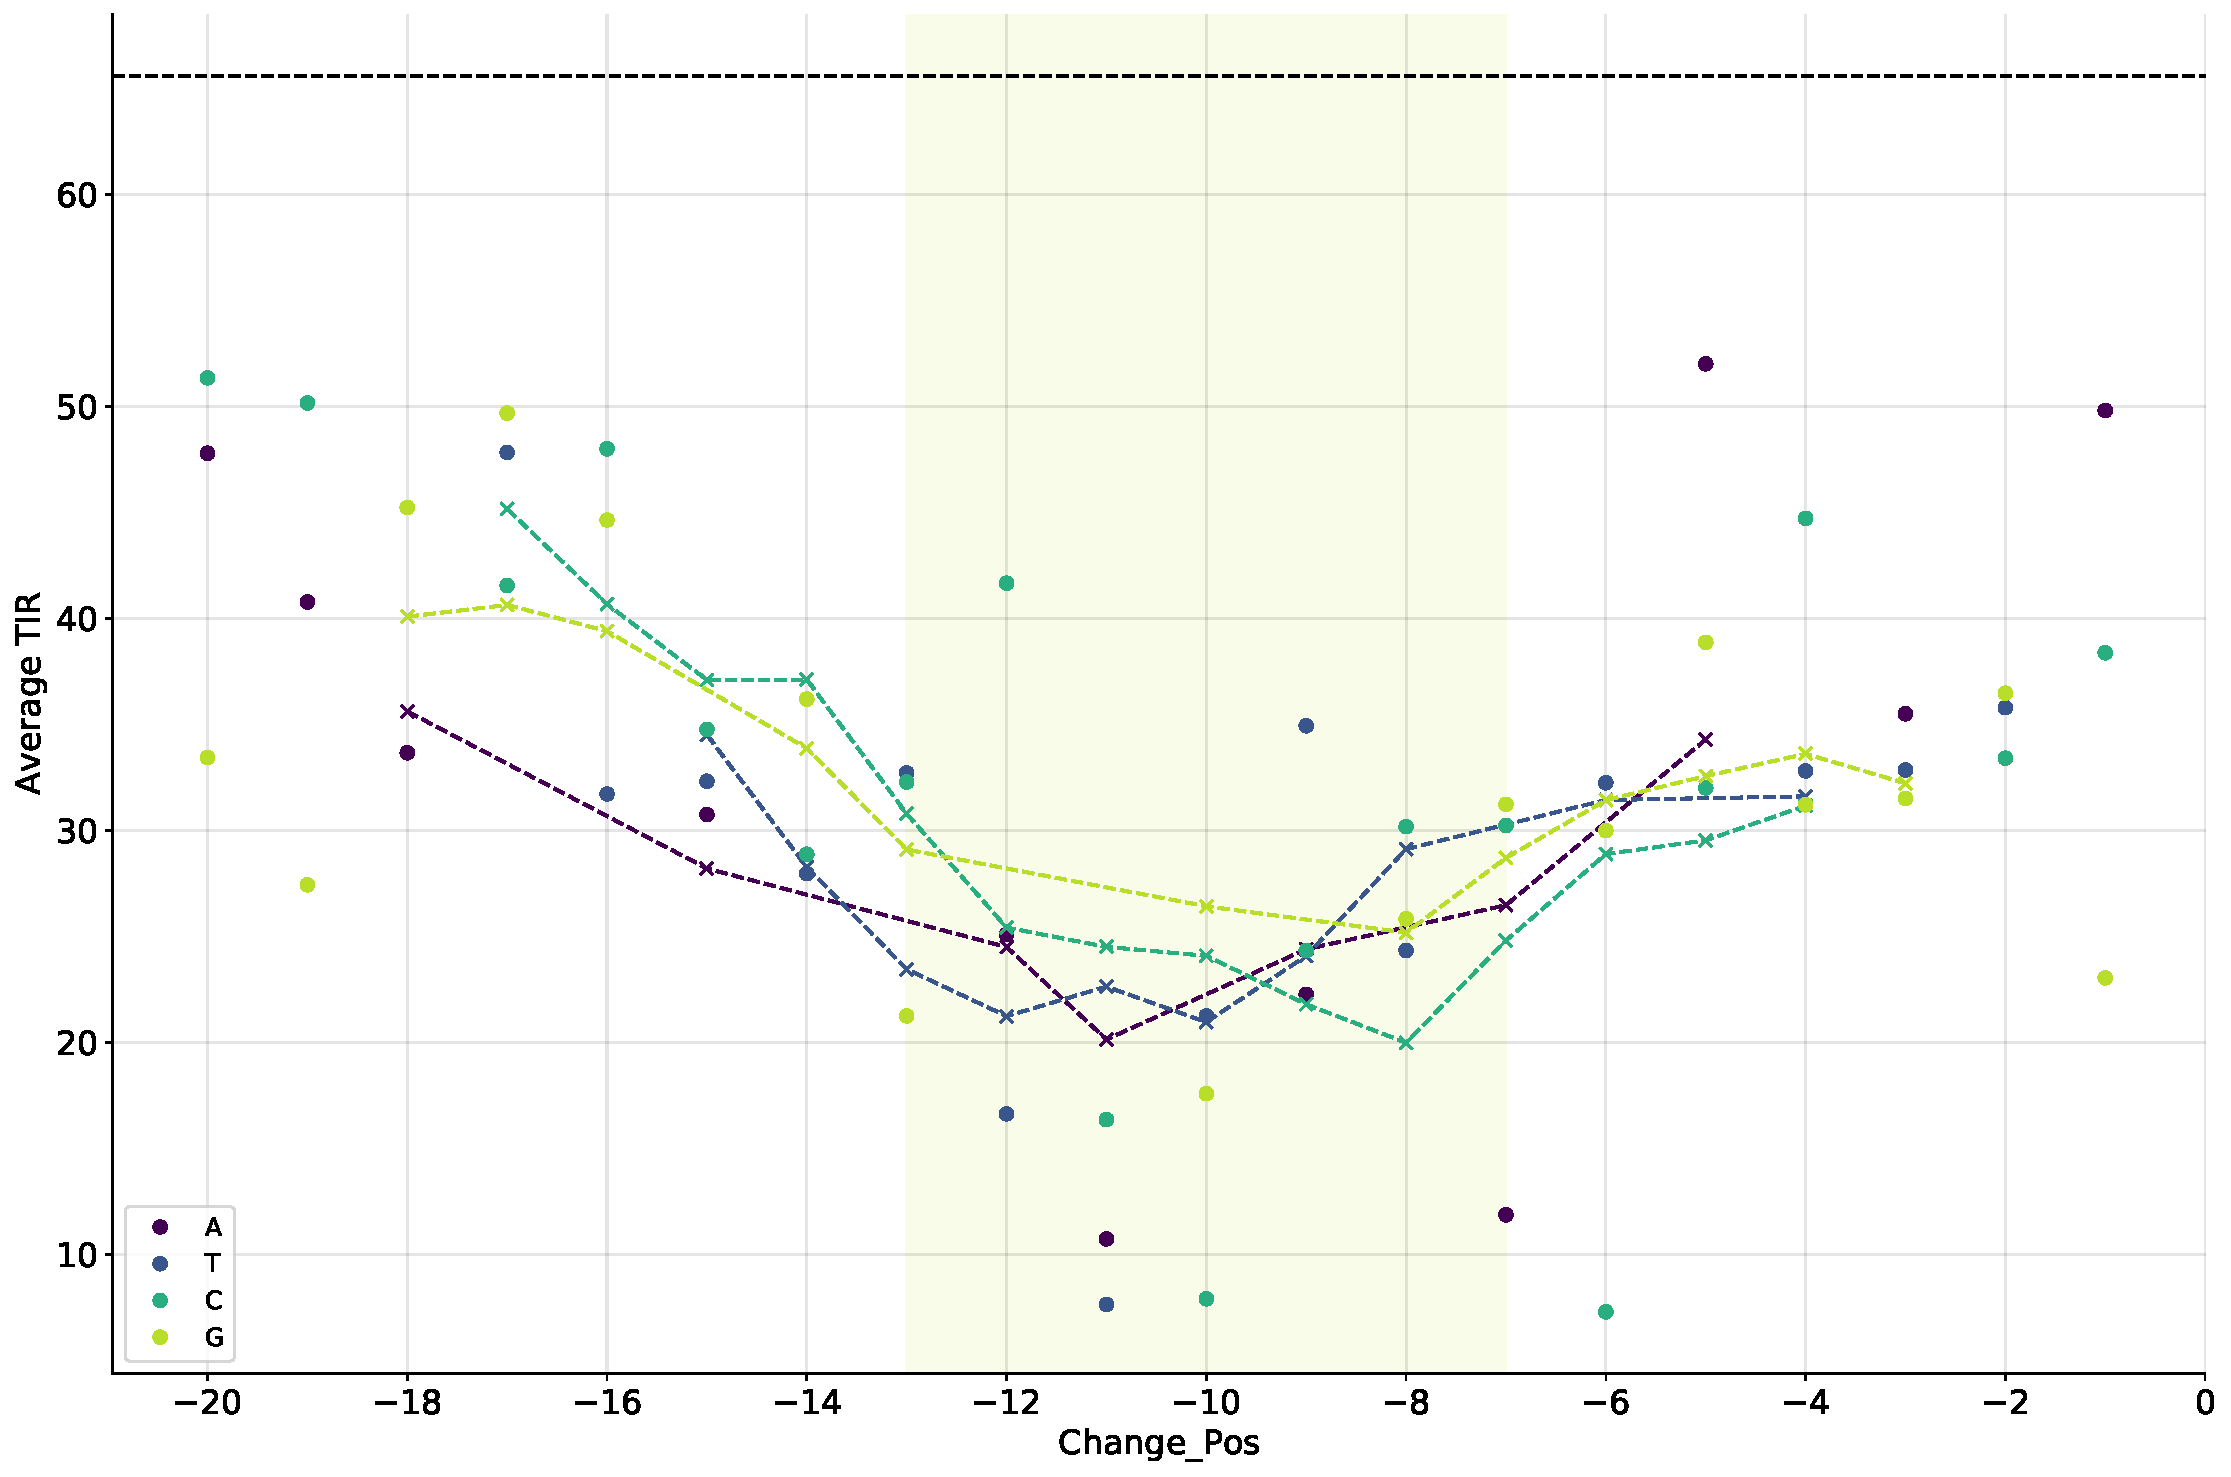
\includegraphics[scale=0.4]{plots/Supplementary/core_vs_noncore.pdf}
    \caption{\textbf{Comparison of base change impact on TIR in core versus non-core region.} The core region is highligthed in light green and the lines are rolling averages for each base. The top dotted line shows the TIR for the benchmark sequence, where dots represent a change at a given position to a given base, which is colour coded.}
    \label{fig:core_vs_noncore}
\end{figure}

\section{Supplementary Figures}

\begin{figure}
     \centering
     \begin{subfigure}[b]{0.49\textwidth}
         \centering
         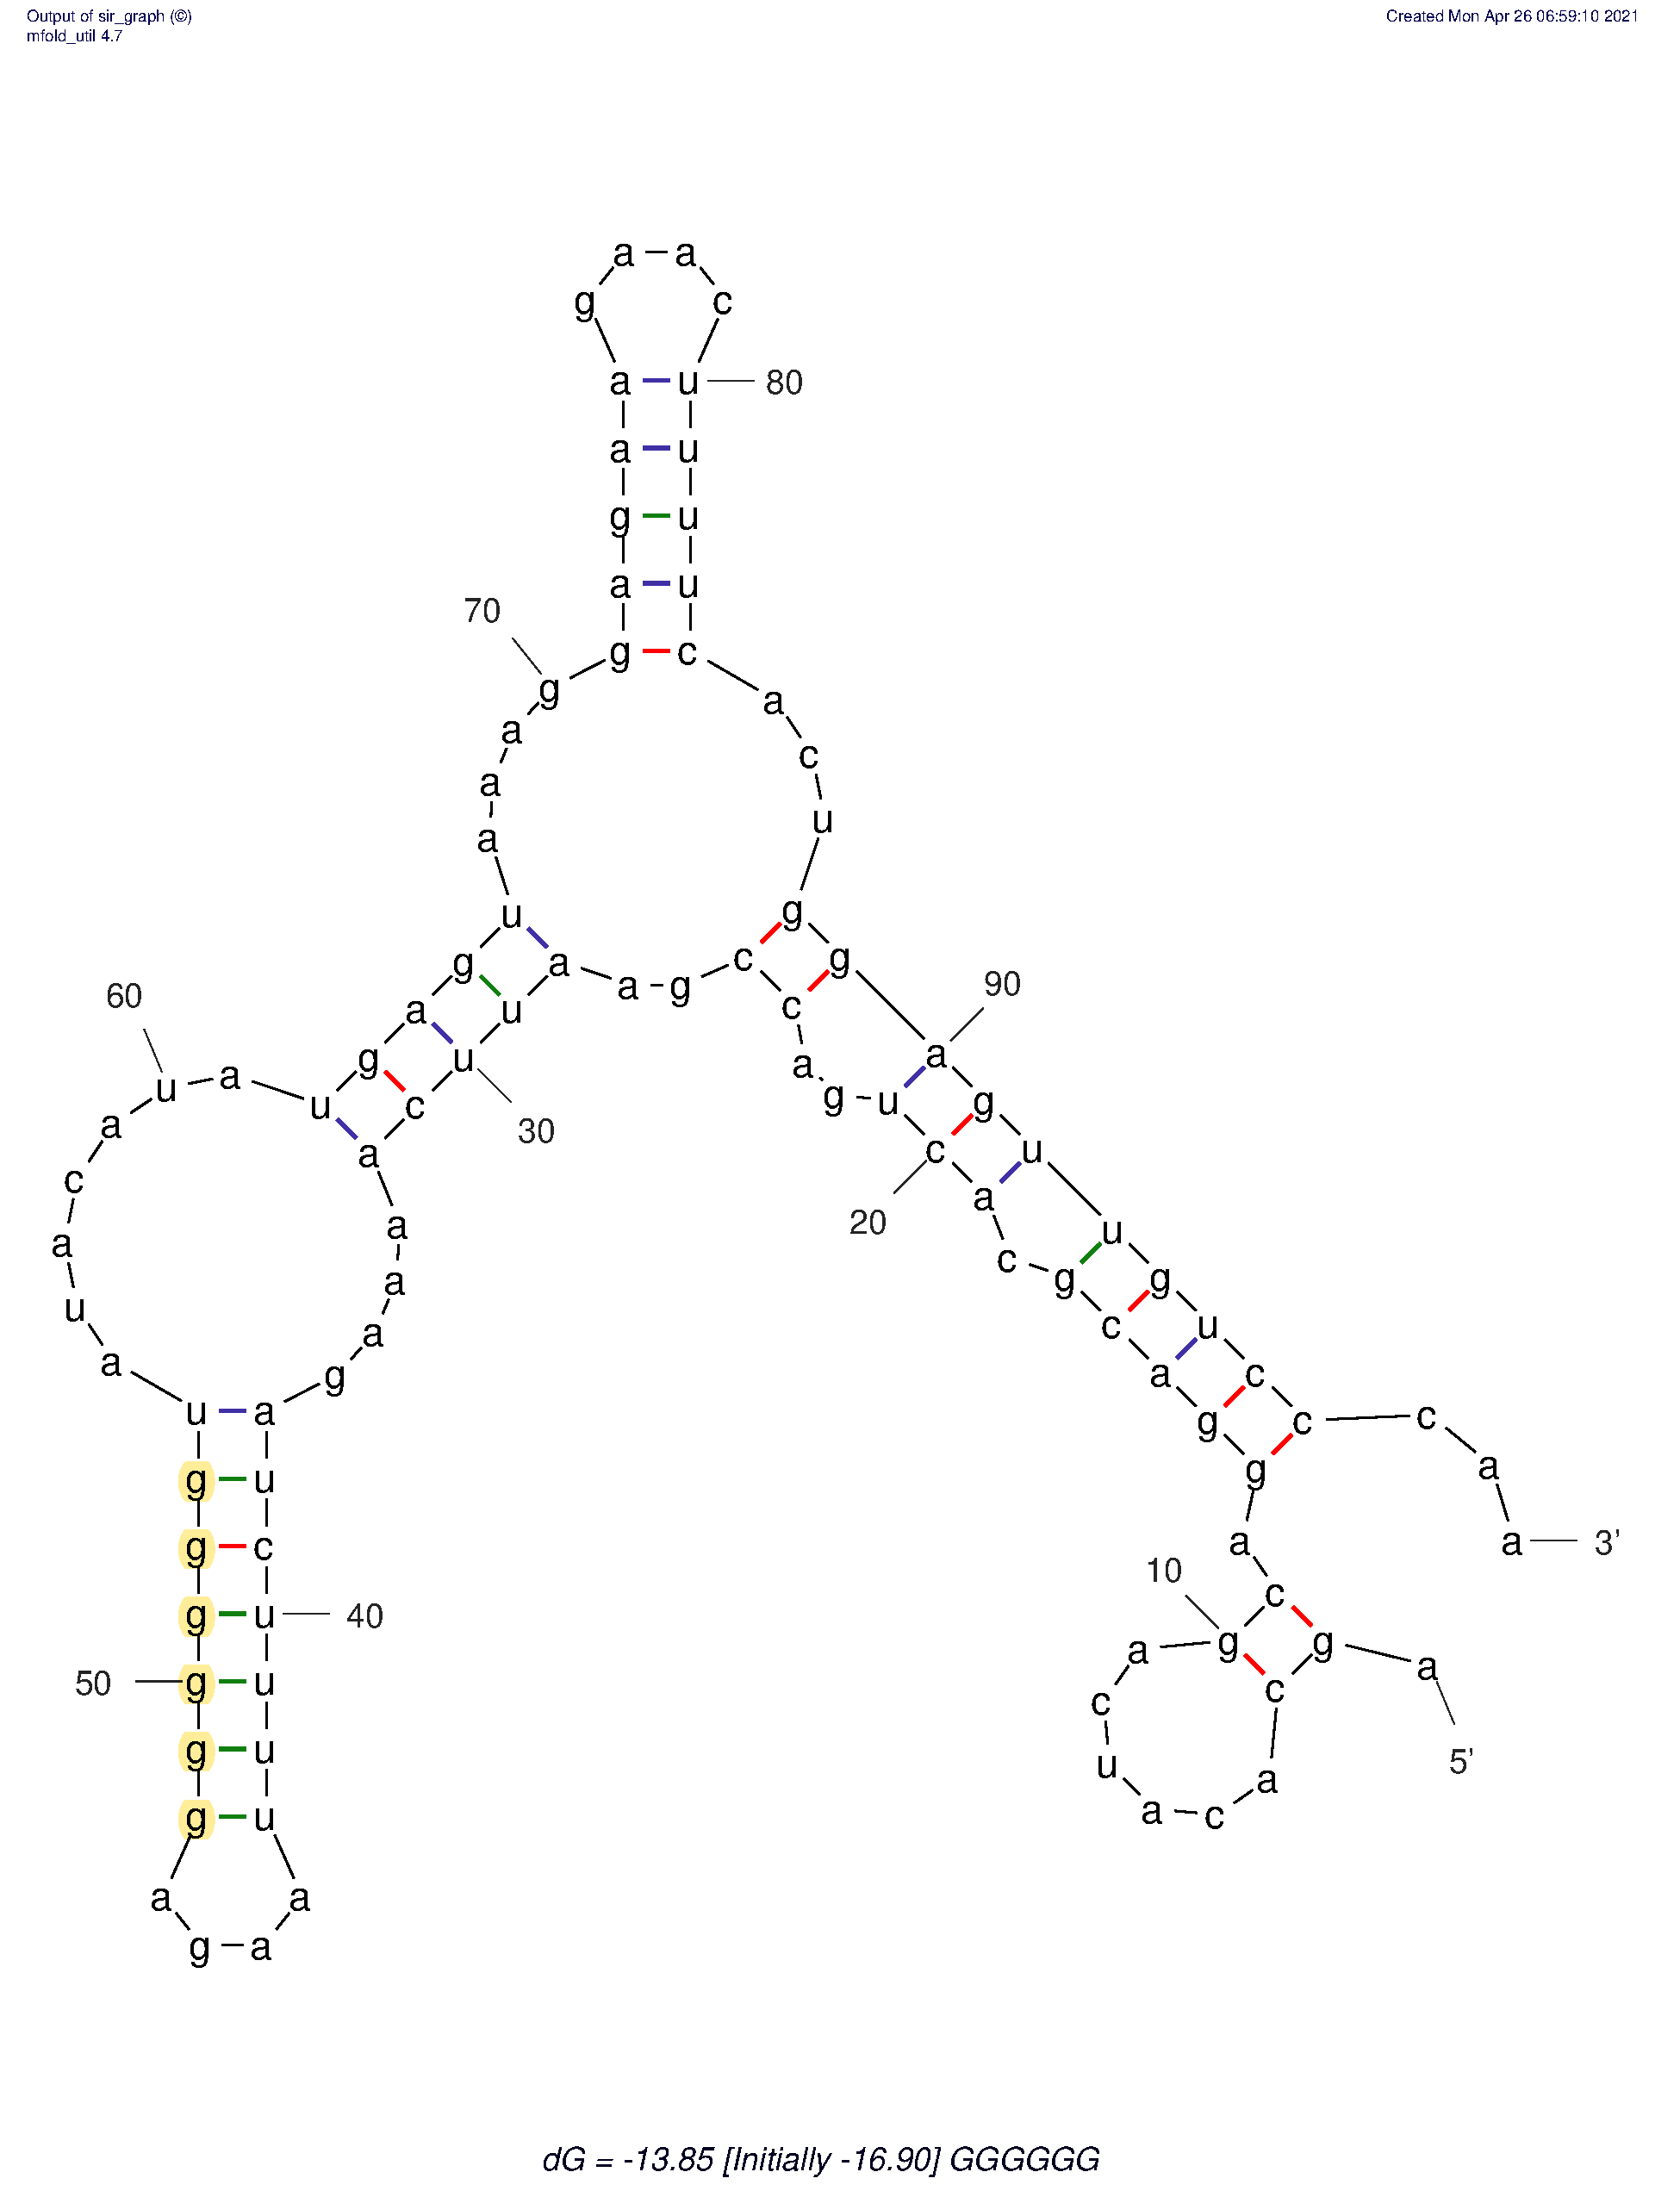
\includegraphics[scale=0.25]{plots/Supplementary/Structure_GGGGGG.pdf}
         \caption{$y=x$}
         \label{fig:GGGGGG}
     \end{subfigure}
     \hfill
     \begin{subfigure}[b]{0.49\textwidth}
         \centering
         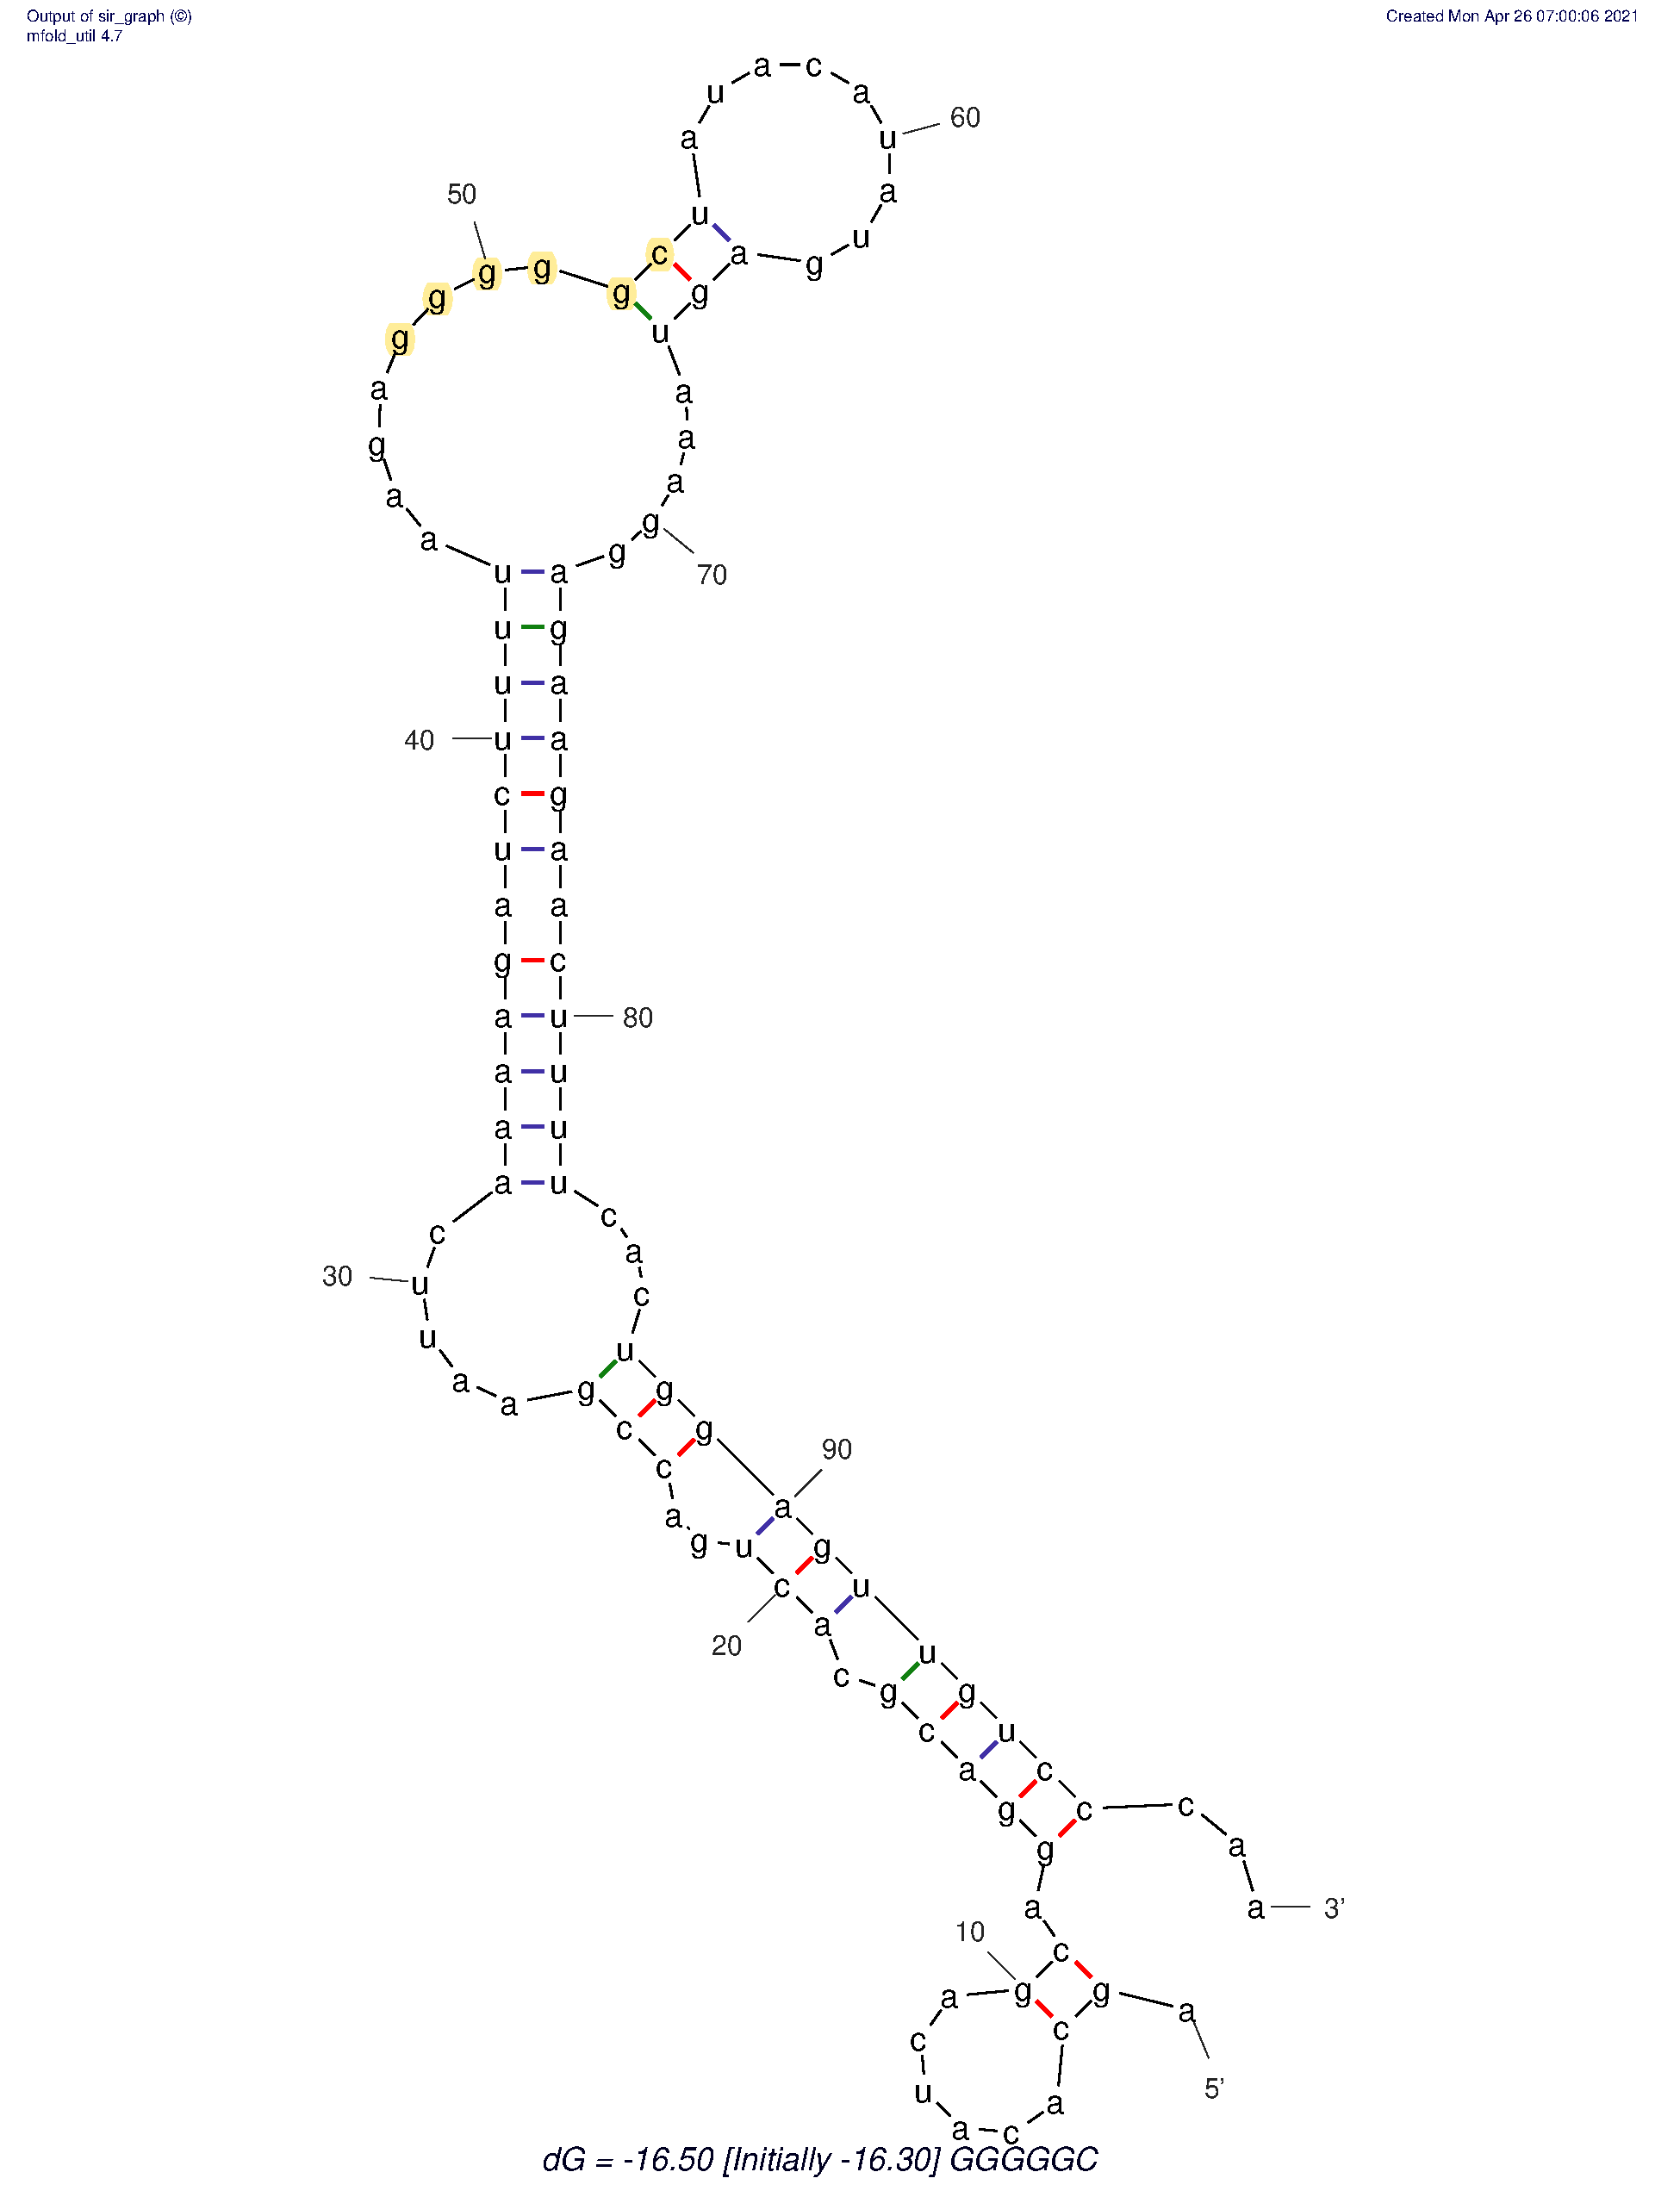
\includegraphics[scale=0.25]{plots/Supplementary/Structure_GGGGGC.pdf}
         \caption{$y=3sinx$}
         \label{fig:GGGGGC}
     \end{subfigure}
     \vskip\baselineskip
     \begin{subfigure}[b]{0.49\textwidth}
         \centering
         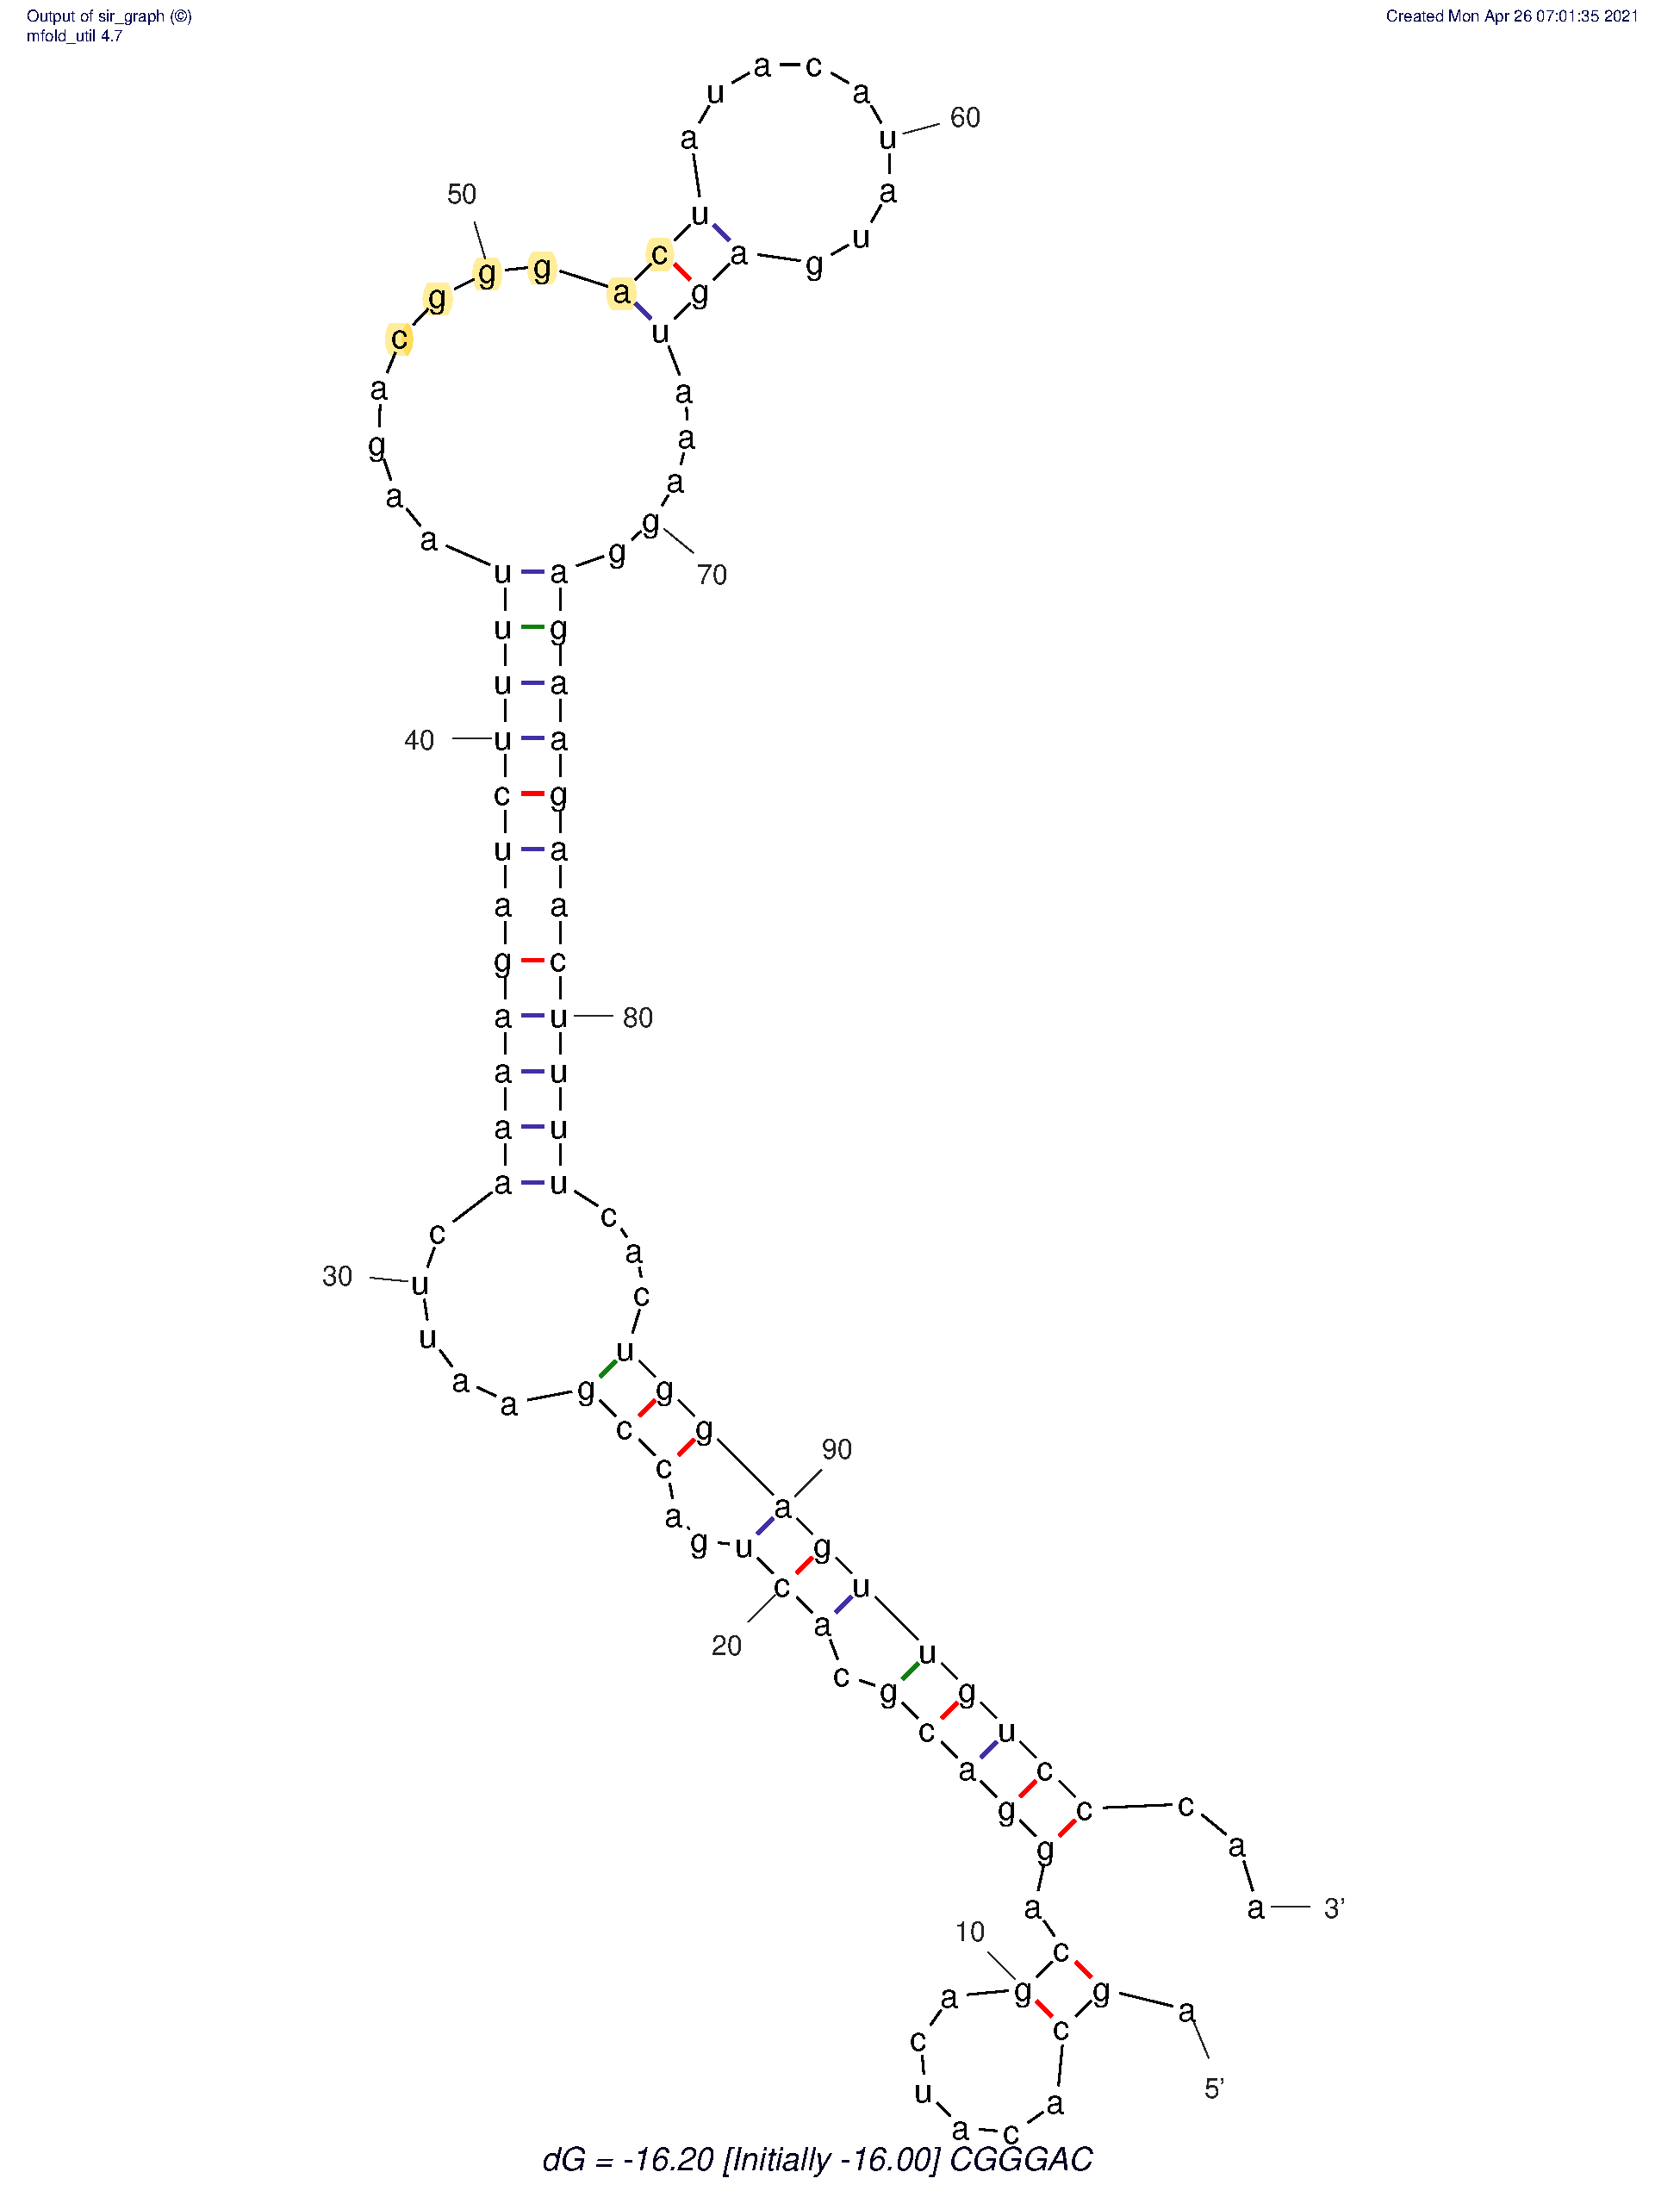
\includegraphics[scale=0.25]{plots/Supplementary/Structure_CGGGAC.pdf}
         \caption{$y=5/x$}
         \label{fig:CGGGAC}
     \end{subfigure}
     \hfill
     \begin{subfigure}[b]{0.49\textwidth}
         \centering
         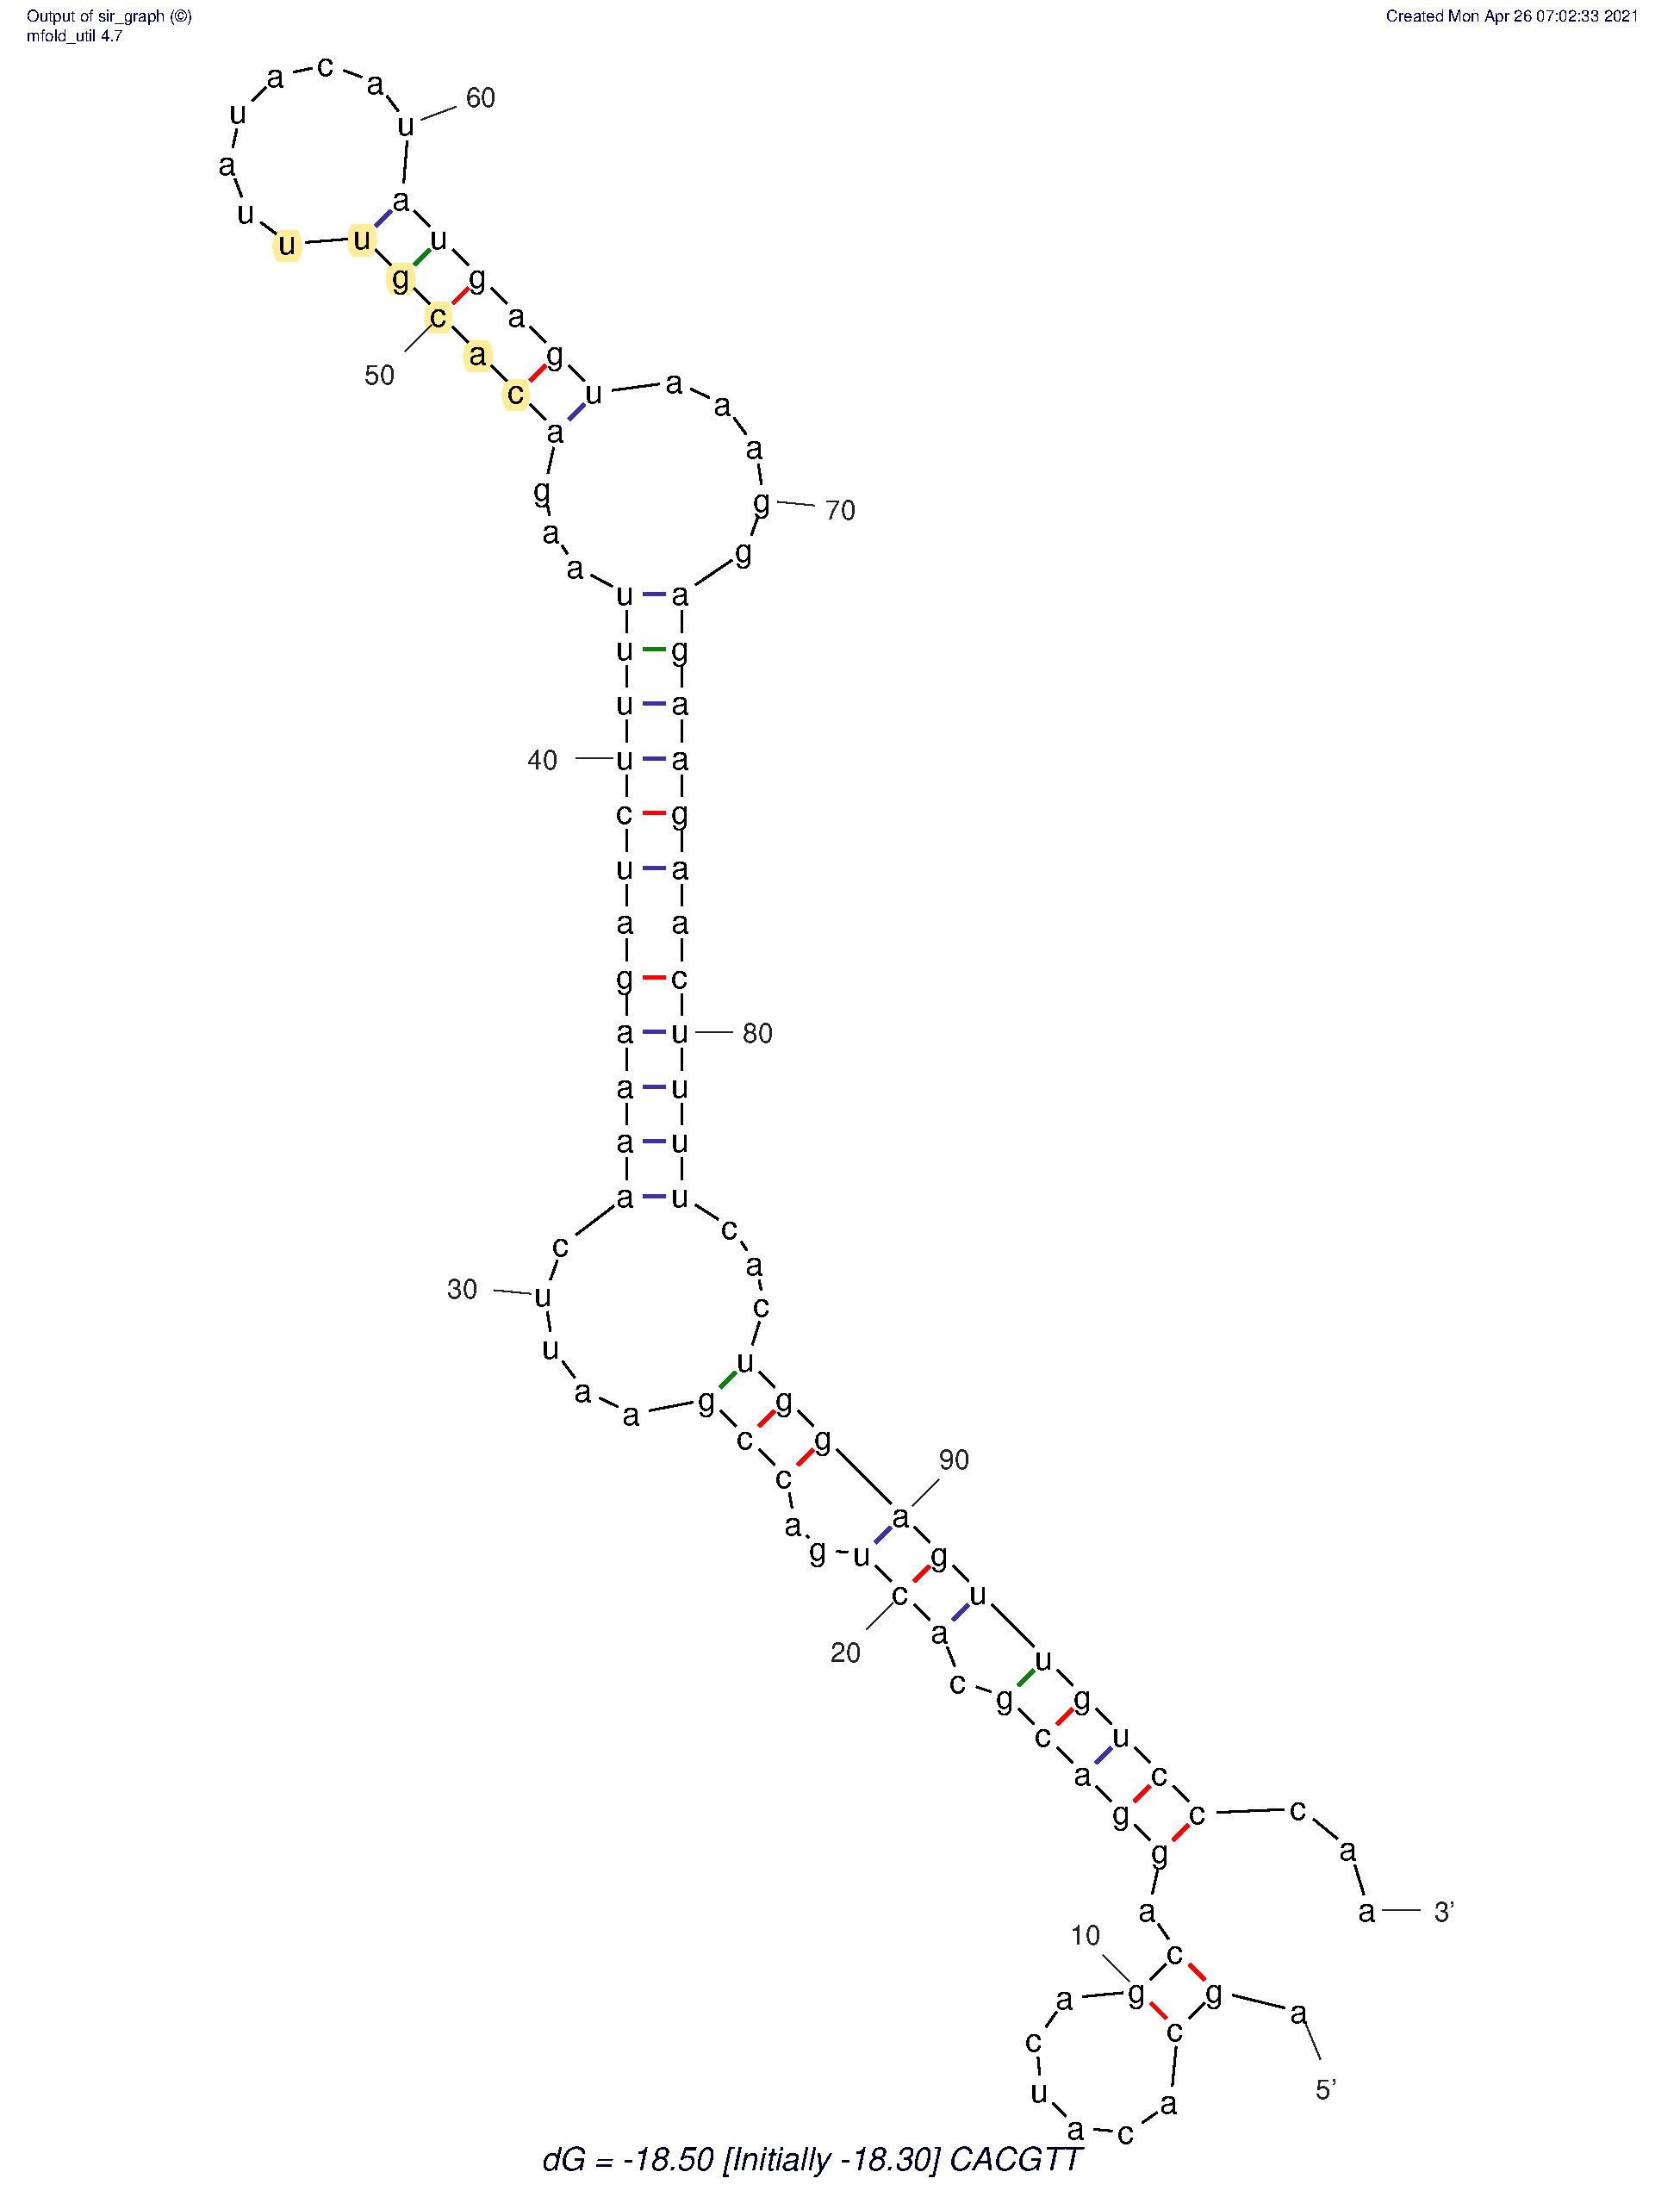
\includegraphics[scale=0.25]{plots/Supplementary/Structure_CACGTT.pdf}
         \caption{$y=5/x$}
         \label{fig:CACGTT}
     \end{subfigure}
        \caption{\textbf{Folding predictionds for four different RBS.} Here we show the predicted, energetically most favourable structures for four of our RBS with the following cores: GGGGGG, GGGGGC, CGGGAC, CACGTT and their immediate upstream and downstream background sequence. There is no discerbile and consistent difference between strong ones (the first two) and weak ones (the last two).}
        \label{fig:structures}
\end{figure}


\newpage

\section{Mixture of Absolute Gaussian}

The raw TIR scores in each round are positive and  have two modes. 
We assume they are mixture of two absolute Gaussian distributions. 
If we can fit the mixture of absolute Gaussian distributions, we can answer the following questions:
\begin{itemize}
    \item is the left peak decreasing in height with each round?
	\item is the left peak going left?
	\item Is the right peak increasing in height with each round?
	\item is the right peak going right?
\end{itemize}

The density of absolute Gaussian (also called \textit{folded normal distribution}) is 
\begin{align}
    f_{Y}\left(x ; \mu, \sigma^{2}\right)=\frac{1}{\sqrt{2 \pi \sigma^{2}}} e^{-\frac{(z-\mu)^{2}}{2 \sigma^{2}}}+\frac{1}{\sqrt{2 \pi \sigma^{2}}} e^{-\frac{(x+\mu)^{2}}{2 \sigma^{2}}}
\end{align}
for $x \geq 0$ and $0$ everywhere else. 
The mean and variance of the absolute Gaussian distribution is 
\begin{align}
    \mu_{Y} &=\sigma \sqrt{\frac{2}{\pi}} \exp \left(\frac{-\mu^{2}}{2 \sigma^{2}}\right)+\mu \operatorname{erf}\left(\frac{\mu}{\sqrt{2 \sigma^{2}}}\right);\\
    \sigma_{Y}^{2} &=\mu^{2}+\sigma^{2}-\mu_{Y}^{2},
\end{align}
where $\operatorname{erf}$ is the error function 
$\operatorname{erf} z=\frac{2}{\sqrt{\pi}} \int_{0}^{z} e^{-t^{2}} d t$.

We consider the model of the mixture of two absolute Gaussian distributions as 
